\section{Physical Basics}
Here the basic definitions, the general models concept, and a list of
models available in \Dumux are given. The actual differential equations
can be found in the local residuals (see Doxygen documentation of the
model's \texttt{LocalResidual} class).

\subsection{Basic Definitions and Assumptions}
Basic definitions and assumptions are given. More information can be found e.g. in \cite{A3:acosta:2006,A3:bielinski:2006}.

\begin{description}
\item[Phases:]
A \emph{phase} is defined as a continuum having distinct properties (e.g. density and viscosity). If phases are miscible, they contain dissolved portions of the substance of the other phase. 
Fluid and solid phases are distinguished. The fluid phases have different affinities to the solid phases. The phase, which has a higher affinity to the solid phases is referred to as the (more) wetting phase. In the case of two phases, the less wetting one is called the nonwetting phase. 

For compositional multi-phase models, fluid phases may be composed of several components, while the solid phases are assumed to consist exclusively of a single component. 

\item[Components:]
The term \emph{component} stands for constituents of the phases which
can be associated with a unique chemical species, or, more generally, with
a group of species exploiting similar physical behavior. For example, Fig. \ref{fig:phaseMassEnergyTransfer} shows a water-gas-NAPL system composed of the phases water (subscript
$\text{w}$), gas ($\text{g}$), and NAPL ($\text{n}$). These phases are
composed of the components water (superscript $\text{w}$), the pseudo-component
air ($\text{a}$), and an organic contaminant ($\text{c}$).

The composition of the components in a phase can influence the phase properties. Furthermore, for mass transfer, the phase behavior is quite different from the component behavior.

\item[Equilibrium:]
For the non-isothermal, multi-phase, multi-component processes in porous media
we state the assumption of \emph{local thermodynamic equilibrium}.
Chemical equilibrium means that the mass/mole fractions of a component in
different phases are in equilibrium.
Thermal equilibrium assumes the same temperature for all considered phases.
Mechanical equilibrium is not valid in a porous medium, since discontinuities
in pressure can occur across a fluid-fluid interface due to capillary effects.

\item[Notation:]
The subscript index $\alpha$, e.g. $\text{w}, \text{n} \text{ and } \text{g}$ in the example of Fig. \ref{fig:phaseMassEnergyTransfer}, refers
to the phase, while the superscript $\kappa$, e.g. $\text{w}, \text{a} \text{ and } \text{c}$ in the example of Fig. \ref{fig:phaseMassEnergyTransfer},
refers to the component.
\end{description}

\begin{table}
\begin{tabular}{llll}
$p_\alpha$ & phase pressure & $\phi$ & porosity \\
$T$ & temperature & $K$ & absolute permeability tensor \\
$S_\alpha$ & phase saturation & $\tau$ & tortuosity \\
$x_\alpha^\kappa$ & mole fraction of component $\kappa$ in phase $\alpha$ & $\boldsymbol{g}$ & gravitational acceleration \\
$X_\alpha^\kappa$ & mass fraction of component $\kappa$ in phase $\alpha$ & $q^\kappa_\alpha$ & volume source term of $\kappa$ in $\alpha$ \\
$\varrho_{\text{mol},\alpha}$ & molar density of phase $\alpha$ & $u_\alpha$ & specific internal energy \\
$\varrho_{\alpha}$ & mass density of phase $\alpha$ & $h_\alpha$ & specific enthalpy \\
$M$ & molar mass of a phase or component & $c_\text{s}$ & specific heat enthalpy \\
$k_{\text{r}\alpha}$ & relative permeability & $\lambda_\text{pm}$ & heat conductivity \\
$\mu_\alpha$ & phase viscosity & $q^h$ & heat source term \\
$D_\alpha^\kappa$ & diffusivity of component $\kappa$ in phase $\alpha$ & $\boldsymbol{v}_{a,\alpha}$  & advective velocity \\
$\boldsymbol{v}_\alpha$ & velocity (Darcy or free flow)& & \\
\end{tabular}
\caption{Notation list for most of the variables and indices used in \Dumux.}

\end{table}

\begin{figure}
  \centering
  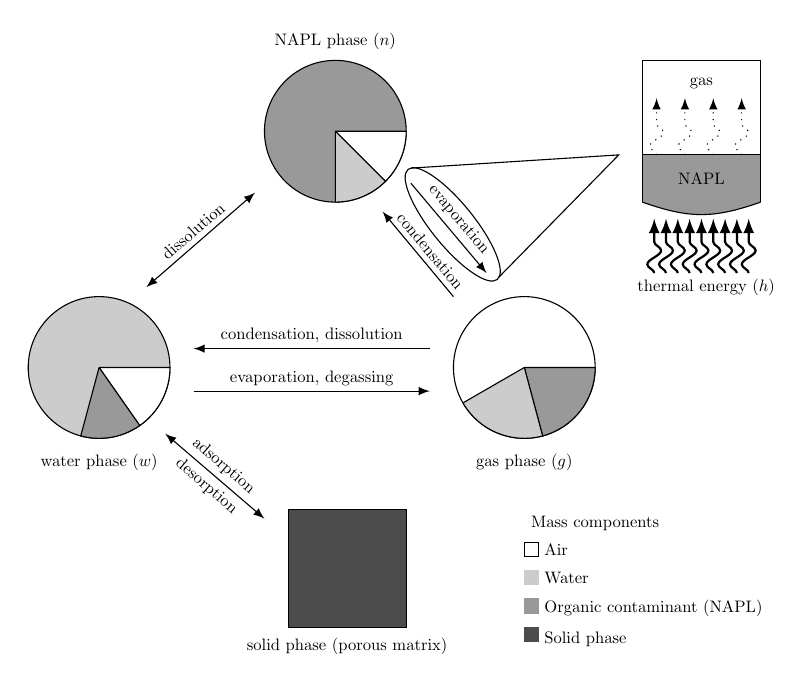
\begin{tikzpicture} [>=latex,scale=0.6, every node/.style={transform shape}]
    % Ellipse 1 solid
    \coordinate (A) at (1,-0.5);
    \draw [fill=black!70](A) rectangle(3.5,2) node at(2.25,-0.9) {solid phase (porous matrix)};
    % Ellipse 2 water
    \coordinate (B) at (-3,5);
    \draw [fill=black!20](B) circle(1.5cm);
    \node [yshift=5mm]at(-3,2.5){water phase $(w)$};
    \draw[fill=white] (B)--+(1.5,0)arc(0:-55:1.5cm)--(B);
    \draw[fill=black!40] (B)--+(-55:1.5cm)arc(-55:-105:1.5cm)--(B);
    % Ellipse 3 gas
    \coordinate (C) at (6,5);
    \draw [](C) circle (1.5cm);
    \node[yshift=5mm]at(6,2.5){gas phase $(g)$};
    \draw [fill=black!40](C)--+(1.5,0)arc(0:-75:1.5cm)--(C);
    \draw [fill=black!20] (C)--+(-75:1.5cm)arc(-75:-150:1.5cm)--(C);
    % Ellipse 4 napl
    \coordinate (D) at (2,10);
    \draw [fill=black!40](D) circle (1.5cm);
    \node[yshift=5mm]at(2,11.4){NAPL phase $(n)$};
    \draw [fill=white](D)--+(1.5,0)arc(0:-45:1.5cm)--(D);
    \draw [fill=black!20] (D)--+(0,-1.5)arc(-90:-45:1.5cm)--(D);
    % arrows
    %A-B
      \draw [<->,white](0.5,1.8)--(-1.6,3.6) node[black,above,sloped,pos=0.5]{adsorption};
      \draw [<->](0.5,1.8)--(-1.6,3.6) node[below,sloped,pos=0.5]{desorption};
    %B-C
      \draw[<-](-1,5.4)--(4,5.4)node[above,sloped,pos=0.5]{condensation, dissolution};
      \draw[->](-1,4.5)--(4,4.5)node[above,sloped,pos=0.5]{evaporation, degassing};
    %B-D
      \draw[<->](-2,6.7)--(0.3,8.7)node[above,sloped,pos=0.5]{dissolution};
    %D-C
      \draw[->](3.6,8.9)--(5.2,7)node[above,sloped,pos=0.5]{evaporation};
      \draw[rotate around={-51:(4,6.8)}](3.35,7.95) ellipse (1.5cm and 0.45cm);  %Ellipse um evaporation
      \draw (3.6,9.22)--(8,9.5)--(5.45,6.9);
      \draw[<-](3,8.3)--(4.5,6.5)node[above,sloped,pos=0.55]{condensation};
    % thermal energy
    \filldraw [black!40](8.5,9.5)rectangle(11,8.5);
    \draw (8.5,9.5)rectangle(11,11.5);
    \draw (8.5,9.5)--(8.5,8.5);
    \draw (11,9.5)--(11,8.5);
    \draw [decorate,decoration={bent,aspect=0.4,amplitude=6},fill=black!40](11,8.5)--(8.5,8.5);
    \foreach \x in {8.75,9,...,10.8}
    \draw [->,decorate,decoration={snake,post length=2mm},thick](\x,7)--(\x,8.15);
    \foreach \x in {8.8,9.4,10,10.6}
    \draw [->,dotted,decorate,decoration={snake,post length=2mm}](\x,9.5)--(\x,10.7);
    \node at(9.75,11){gas};
    \node at(9.75,9){NAPL};
    \node at(9.85,6.7){thermal energy $(h)$};
    % legende
    \node at (7.5,1.7){Mass components};
    \draw[](6,1)rectangle +(0.3,0.3) node at(6.3,1.15) [right]{Air};
    \filldraw[black!20](6,0.4) rectangle +(0.3,0.3) node at (6.3,0.55)[black,right]{Water};
    \filldraw[black!40](6,-0.2) rectangle +(0.3,0.3) node at (6.3,-0.1)[right,black]{Organic contaminant (NAPL)};
    \filldraw[black!70](6,-0.8) rectangle +(0.3,0.3) node at (6.3,-0.75)[right,black]{Solid phase};
  \end{tikzpicture}
  \caption{Mass and energy transfer between the phases in a water-NAPL-gas system \cite{A3:class:2002a}}
  \label{fig:phaseMassEnergyTransfer}
\end{figure}

\subsection[Scale]{Scale\footnote{\label{foot:hommel}This subsection is taken from \cite{hommel2016modeling} in a slightly adapted form.}} 

Depending on the scale of interest, physical and chemical processes and properties can be described 
using different approaches. 
On the molecular scale, the properties and interactions of individual molecules are described, 
which is only feasible for a restricted number of molecules. 
For larger systems, a continuum approach is used, where properties are averaged over 
groups of similar molecules, assuming continuous matter. This upscaling by averaging 
from the molecular scale results in the micro-scale, on which the system is described by
the pore geometry and the distribution of distinct fluid phases within the pores. 
However, for larger laboratory or field-scale applications, the micro-scale is still 
computationally prohibitively expensive and system descriptions on the macro-scale 
are used for calculations. The macro-scale description is obtained by averaging over the 
micro-scale properties within a representative elementary volume (REV), 
which needs to be large enough to ensure that the averaged properties are independent of the REV size 
or position. However, it should in turn be much smaller than the entire domain size \citep{helmig1997multiphase}. %(Bear 1988)
The detailed pore-geometry and phase-distribution information of the micro-scale is lost
on the macro-scale and replaced by volume average quantities, 
such as porosity, permeability and phase saturation, 
and relations like the Darcy's law.
The macro-scale is also called the REV (or Darcy) scale and is the scale of the 
models available in \Dumux.

\subsection[Porous medium properties]{Porous medium properties\footref{foot:hommel}}
\subsubsection{Porosity}
The porosity $\phi$ is defined as the fraction of the volume occupied by fluids in an REV $V_\mathrm{fluid}$ 
divided by the total volume of the REV $V_\mathrm{total}$.

\begin{equation}\label{eq:def_poro}
\phi=\frac{V_\mathrm{fluid}}{V_\mathrm{total}}=1-\frac{V_\mathrm{solid}}{V_\mathrm{total}}.
\end{equation}


\subsubsection{Intrinsic permeability} 
The intrinsic permeability is a measure on the REV scale of the ease of fluid flow through porous media. 
It relates the potential gradient and the resulting flow velocity in the Darcy equation. 
As the porous medium may have a structure leading to preferential flow in certain directions, 
intrinsic permeability is in general a tensorial quantity $\mathbf{K}$. 
For isotropic porous media, it can be reduced to a scalar quantity $K$.

% \begin{equation}
%  \mathbf{v}=
% \end{equation}

\newpage
\subsection[Mass fraction, mole fraction]{Mass fraction, mole fraction\footref{foot:hommel}}\label{sec:mole_frac_molality}
The composition of a phase is described by mass or mole fractions of the components. 
The mole fraction $x^\kappa_\alpha$ of component $\kappa$ in phase $\alpha$ is defined as:

\begin{equation}\label{eq:def_molefrac}
x^\kappa_\alpha = \frac{n^\kappa_\alpha}{\sum_i n^i_\alpha},
\end{equation}

where $n^\kappa_\alpha$ is the number of moles of component $\kappa$ in phase $\alpha$. 
The mass fraction $X^\kappa_\alpha$ is defined similarly 
using the mass of component $\kappa$ in phase $\alpha$ instead of $n^\kappa_\alpha$,
$X^\kappa_\alpha = \nicefrac{\mathrm{mass^\kappa_\alpha}}{\mathrm{mass^{total}_\alpha}}$.
% as:
% 
% \begin{equation}\label{eq:def_massfrac}
% X^\kappa_\alpha = \frac{m^\kappa_\alpha}{\sum_i m^i_\alpha},
% \end{equation}
% 
% where $m^\kappa_\alpha$ is the mass of component $\kappa$ in phase $\alpha$. 
The molar mass $M^\kappa$ of the component $\kappa$ relates the mass fraction 
to the mole fraction and vice versa.

\subsection[Fluid properties]{Fluid properties\footref{foot:hommel}}\label{sec:fluid_properties}
The most important fluid properties to describe fluid flow on the REV scale are density and viscosity.

\subsubsection{Density}\label{sec:density}
The density $\rho_\alpha$ of a fluid phase $\alpha$ is defined as the ratio of its mass to its volume
$(\rho_\alpha = \nicefrac{\mathrm{mass_\alpha}}{\mathrm{volume_\alpha}})$ while 
the molar density $\rho_{\mathrm{mol},\alpha}$ is defined as the ratio of the number of moles per volume 
$(\rho_{\mathrm{mol},\alpha} = \nicefrac{\mathrm{moles_\alpha}}{\mathrm{volume_\alpha}})$.

\subsubsection{Viscosity}\label{sec:viscosity}
The dynamic viscosity $\mu_\alpha$ characterizes the resistance of a fluid to flow. 
As density, it is a fluid phase property.  
For Newtonian fluids, it relates the shear stress $\tau_\mathrm{s}$ to the  
velocity gradient $\nicefrac{d v_{\alpha,\,x}}{d y}$: 

\begin{equation}\label{eq:def_viscosity}
\tau_\mathrm{s} = \mu_\alpha \frac{d v_{\alpha,\,x}}{d y}.
\end{equation}

Density and viscosity are both dependent on pressure, temperature and phase composition. 

\subsection[Fluid phase interactions in porous media]{Fluid phase interactions in porous media\footref{foot:hommel}}\label{sec:fluid_interact}
If more than a single fluid is present in the porous medium, the fluids interact with each other and the solids, which leads to additional properties for multi-phase systems. 

\subsubsection{Saturation}\label{sec:saturation}
The saturation $S_\alpha$ of a phase $\alpha$ is defined as the ratio of the volume occupied 
by that phase to the total pore volume within an REV. 
As all pores are filled with some fluid, the sum of the saturations of all present phases is equal to one.

\subsubsection{Capillary pressure}\label{sec:pc}
Immiscible fluids form a sharp interface as a result of differences in their intermolecular forces 
translating into different adhesive and cohesive forces at the fluid-fluid and fluid-fluid-solid interfaces 
creating interfacial tension on the microscale. 
From the mechanical equilibrium which has also to be satisfied at the interface, 
a difference between the pressures of the fluid phases results defined as 
the capillary pressure $p_\mathrm{c}$:  

\begin{equation}\label{eq:pc-pn_pw}
p_\mathrm{c} = p_\mathrm{n} - p_\mathrm{w}.
\end{equation}

On the microscale, $p_\mathrm{c}$ can be calculated from the surface tension 
according to the Laplace equation \citep[see][]{helmig1997multiphase}.

On the REV scale, however, capillary pressure needs to be defined by quantities of that scale. 
Several empirical relations provide expressions to link $p_\mathrm{c}$ to the wetting-phase saturation $S_\mathrm{w}$. 
An example is the relation given by \citet{brooks1964hydrau} %, Corey1994} 
to determine $p_\mathrm{c}$ based on 
$S_\mathrm{e}$, which is the effective wetting-phase saturation,
the entry pressure $p_\mathrm{d}$, and the parameter $\lambda$ describing the pore-size distribution:

\begin{equation}\label{eq:pc-Sw}
p_\mathrm{c} = p_\mathrm{d} S_\mathrm{e}^{-\frac{1}{\lambda}},
\end{equation}

with 

\begin{equation}\label{eq:Se}
S_\mathrm{e} = \frac{S_\mathrm{w}-S_\mathrm{w,r}}{1-S_\mathrm{w,r}},
\end{equation}

where $S_\mathrm{w,r}$ is the residual wetting phase saturation which cannot be displaced
by another fluid phase and remains in the porous medium.

\subsubsection{Relative permeability}\label{sec:kr}
The presence of two fluid phases in the porous medium reduces the space available for flow 
for each of the fluid phases. 
This increases the resistance to flow of the phases, which is accounted for by the means of 
the relative permeability $k_\mathrm{r,\alpha}$, which scales the intrinsic permeability. 
It is a value between zero and one, depending on the saturation. 
The relations describing the relative permeabilities of the wetting and nonwetting phase are different 
as the wetting phase predominantly occupies small pores and the edges of larger pores while the 
nonwetting phases occupies large pores.
The relative permeabilities for the wetting phase $k_\mathrm{r,w}$ and the nonwetting phase are e.g. calculated as (also by \citet{brooks1964hydrau}):

\begin{equation}\label{eq:krw}
k_\mathrm{r,w} = S_\mathrm{e}^{\frac{2+3\lambda}{\lambda}}
\end{equation}
and  
\begin{equation}\label{eq:krn}
k_\mathrm{r,n} = \left( 1- S_\mathrm{e}\right)^2 \left( 1- S_\mathrm{e}^{\frac{2+\lambda}{\lambda}}\right).
\end{equation}

\subsection[Transport processes in porous media]{Transport processes in porous media \footref{foot:hommel}}\label{sec:tipm}
On the macro-scale, the transport of mass can be grouped according to the driving force of the 
transport process. Pressure gradients result in the advective transport of a fluid phase
and all the components constituting the phase, 
while concentration gradients result in the diffusion of a component within a phase. 

\subsubsection{Advection}\label{sec:Advection}
Advective transport is determined by the flow field. 
On the macro-scale, the velocity $\mathbf{v}$ is calculated using the Darcy equation
depending on the potential gradient $(\nabla p_\alpha - \rho_\alpha \mathbf{g})$, 
accounting for both pressure difference and gravitation, 
the intrinsic permeability of the porous medium, 
and the viscosity $\mu$ of the fluid phase:

\begin{equation} \label{eq:Darcy1p}
\mathbf{v}=-\frac{\mathbf{K}}{\mu}(\nabla p - \rho \mathbf{g}).
\end{equation}

$\mathbf{v}$ is proportional to $(\nabla p - \rho \mathbf{g})$ with the proportional factor $\nicefrac{\mathbf{K}}{\mu}$.
This equation can be extended to calculate the velocity $\mathbf{v}_{\alpha}$ of phase $\alpha$ in the case of
two-phase flow by considering the relative permeability $k_\mathrm{r,\alpha}$ (Section~\ref{sec:kr}):

\begin{equation} \label{eq:Darcy2p}
\mathbf{v}_{\alpha}=-\frac{k_\mathrm{r,\alpha}\mathbf{K}}{\mu_{\alpha}}(\nabla p_{\alpha} - \rho_{\alpha} \mathbf{g})
\end{equation}

\subsubsection{Diffusion}\label{sec:Diffusion}
Molecular diffusion is a process determined by the concentration gradient.
It is commonly modeled as Fickian diffusion following Fick's first law:

\begin{equation} \label{eq:Diffusion}
\mathbf{j_d}=-\rho_{\alpha} D^\kappa_\alpha \nabla X^\kappa_\alpha,
\end{equation}

where $D^\kappa_\alpha$ is the molecular diffusion coefficient of component $\kappa$ in phase $\alpha$.
In a porous medium, the actual path lines are tortuous due to the impact of the solid matrix.
This tortuosity and the impact of the presence of multiple fluid phases
is accounted for by using an effective diffusion coefficient $D^\kappa_\mathrm{pm, \alpha}$:

\begin{equation} \label{eq:diffusion_coeff_pm}
D^\kappa_\mathrm{pm, \alpha}= \phi \tau_\alpha S_\alpha D^\kappa_\alpha,
\end{equation}

where $\tau_\alpha$ is the tortuosity of phase $\alpha$.

\subsection{Gas mixing laws}
Prediction of the $p-\varrho-T$ behavior of gas mixtures is typically based on two (contradicting) concepts: Dalton's law or Amagat's law.
In the following the two concepts will be explained in more detail.
%
\subsubsection{Dalton's law}
Dalton's law assumes that the gases in the mixture are non-interacting (with each other) and each gas independently applies its own pressure (partial pressure), the sum of which is the total pressure:
%
\begin{equation}
p = \sum_{i}^{}p_i.
\end{equation}
Here $p_i$ refers to the partial pressure of component i.
As an example, if two equal volumes of gas A and gas B are mixed, the volume of the mixture stays the same but the pressures add up (see Figure \ref{fig:dalton1}).
%
\begin{figure}[ht]
  \centering
  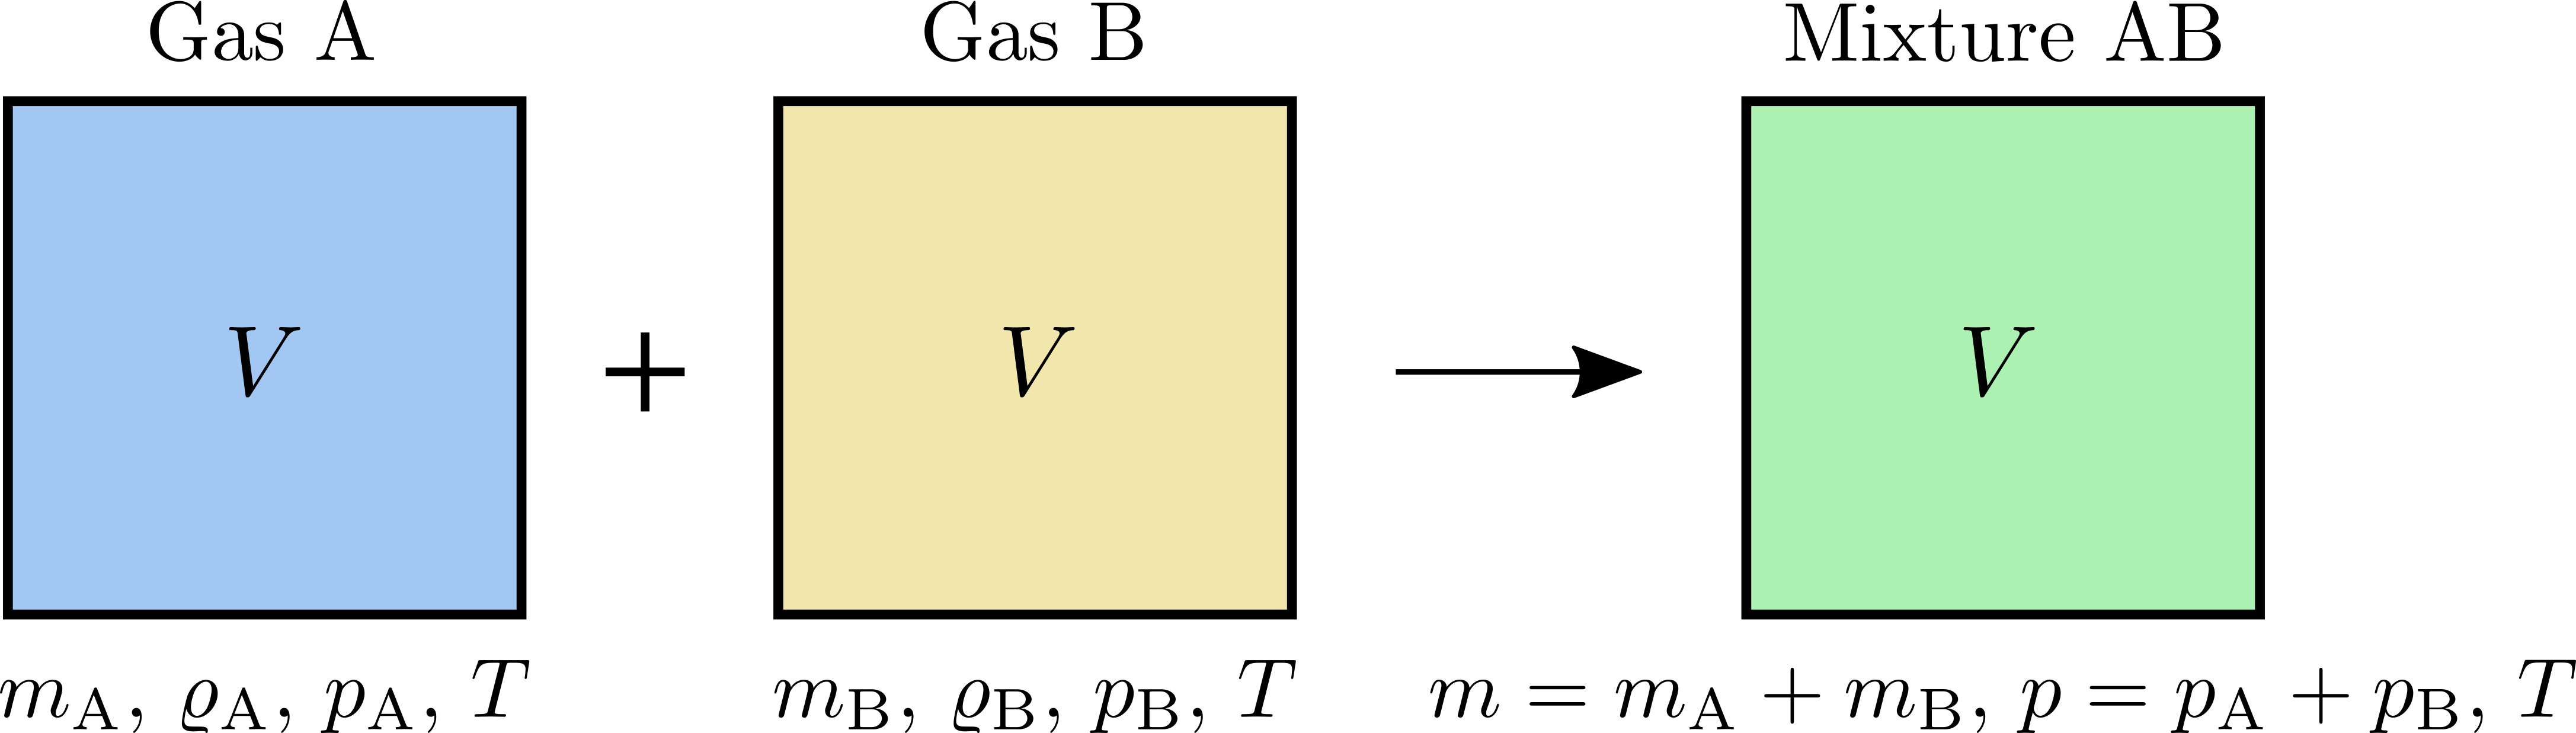
\includegraphics[width=0.7\textwidth]{png/dalton1.png}
  \caption{Dalton's law visualized}
  \label{fig:dalton1}
\end{figure}
%
The density of the mixture, $\varrho$, can be calculated as follows:
\begin{equation}
\varrho = \frac{m}{V} = \frac{m_\mathrm{A} + m_\mathrm{B}}{V} = \frac{\varrho_\mathrm{A} V + \varrho_\mathrm{B} V}{V} = \varrho_\mathrm{A} + \varrho_\mathrm{B},
\end{equation}
%
or for an arbitrary number of gases:
\begin{equation}
\varrho = \sum_{i}^{} \varrho_i ; \quad \varrho_m = \sum_{i}^{} \varrho_{m,i}.
\end{equation}
%
\subsubsection{Amagat's law}
Amagat's law assumes that the volumes of the component gases are additive; the interactions of the different gases are the same as the average interactions of the components. This is known as Amagat's law:
%
\begin{equation}
V = \sum_{i}^{}V_i.
\end{equation}
%
As an example, if two volumes of gas A and B at equal pressure are mixed, the pressure of the mixture stays the same, but the volumes add up (see Figure \ref{fig:dalton2}).
%
\begin{figure}[ht]
  \centering
  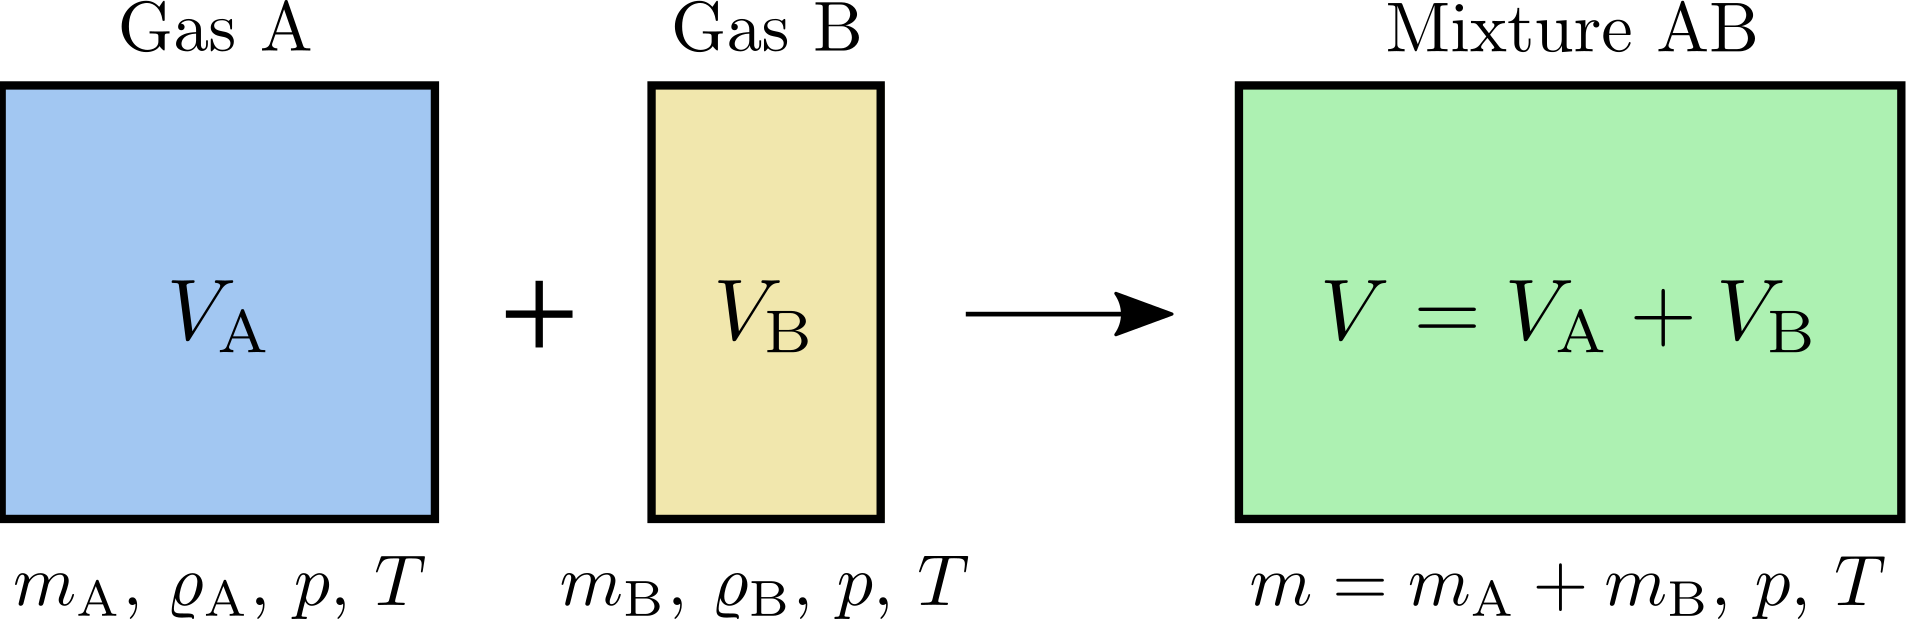
\includegraphics[width=0.7\textwidth]{png/dalton2.png}
  \caption{Amagat's law visualized}
  \label{fig:dalton2}
\end{figure}
%
The density of the mixture, $\varrho$, can be calculated as follows:
\begin{equation}
\varrho = \frac{m}{V} = \frac{m}{V_\mathrm{A} + V_\mathrm{B}} = \frac{m}{\frac{m_\mathrm{A}}{\varrho_\mathrm{A}} \frac{m_\mathrm{B}}{\varrho_\mathrm{B}}} =
\frac{m}{\frac{X_\mathrm{A} m}{\varrho_\mathrm{A}} \frac{X_\mathrm{B} m}{\varrho_\mathrm{B}}} = \frac{1}{\frac{X_\mathrm{A}}{\varrho_\mathrm{A}} \frac{X_\mathrm{B}}{\varrho_\mathrm{B}}},
\end{equation}
%
or for an arbitrary number of gases:
%
\begin{equation}
\varrho = \frac{1}{\sum_{i}^{}\frac{X_i}{\varrho_i}}  ; \quad  \varrho_m = \frac{1}{\sum_{i}^{}\frac{x_i}{\varrho_{m,i}}}.
\end{equation}
%
\subsubsection{Ideal gases}
An ideal gas is defined as a gas whose molecules are spaced so far apart that the behavior of a molecule is not influenced by the presence of other molecules.
This assumption is usually valid at low pressures and high temperatures. The ideal gas law states that, for one gas:
%
\begin{equation}
p = \varrho \frac{RT}{M} ; \quad p= \varrho_m RT.
\end{equation}
%
Using the assumption of ideal gases and either Dalton's law or Amagat's law lead to the density of the mixture, $\varrho$, as:
%
\begin{equation}
\varrho = \frac{p}{RT} \sum_{i}^{}M_i x_i ; \quad \varrho_m = \frac{p}{RT}.
\end{equation}
%
\subsection{Available Models}
A list of all available models can be found
in the Doxygen documentation at
\url{http://www.dumux.org/doxygen-stable/html-\DumuxVersion/modules.php}.
The documentation includes a detailed description for every model.
